\documentclass[12pt, hidelinks]{article}
\usepackage[brazil]{babel}
\usepackage[utf8]{inputenc}
\usepackage{amsmath}
\usepackage{natbib}
\usepackage{listings}
\usepackage{color}

\definecolor{codegreen}{rgb}{0,0.6,0}
\definecolor{codegray}{rgb}{0.5,0.5,0.5}
\definecolor{codepurple}{rgb}{0.58,0,0.82}
\definecolor{backcolour}{rgb}{0.95,0.95,0.92}

\lstdefinestyle{mystyle}{
  backgroundcolor=\color{backcolour},
  commentstyle=\color{codegreen},
  keywordstyle=\color{red},
  numberstyle=\tiny\color{codegray},
  stringstyle=\color{codepurple},
  basicstyle=\footnotesize,
  breakatwhitespace=false,
  breaklines=true,
  captionpos=b,
  keepspaces=true,
  numbers=left,
  numbersep=5pt,
  showspaces=false,
  showstringspaces=false,
  showtabs=false,
  tabsize=2,
  extendedchars=true,
  literate={á}{{\'a}}1 {ã}{{\~a}}1 {õ}{{\~o}}1 {é}{{\'e}}1 {ç}{{\c{c}}}1,
}

\lstset{style=mystyle}
\usepackage{url}
\usepackage{amsmath}
\usepackage{float}
\usepackage{graphicx}
\graphicspath{{images/}}
\usepackage{parskip}
\usepackage{fancyhdr}
\usepackage{vmargin}
\usepackage{hyperref}
\setmarginsrb{3 cm}{2.5 cm}{3 cm}{2.5 cm}{1 cm}{1.5 cm}{1 cm}{1.5 cm}


\title{Resolução de Equações Diferenciais}         % Title
\author{Wilton Rodrigues}								% Author
\date{\today}											      % Date

\makeatletter
\let\thetitle\@title
\let\theauthor\@author
\let\thedate\@date
\makeatother

\pagestyle{fancy}
\fancyhf{}
\lhead{\centering{\thetitle}}
\cfoot{\thepage}

\begin{document}

%%%%%%%%%%%%%%%%%%%%%%%%%%%%%%%%%%%%%%%%%%%%%%%%%%%%%%%%%%%%%%%%%%%%%%%%%%%%%%%%%%%%%%%%%

\begin{titlepage}
  \centering
  \begin{figure}[H]
    \centering
    
\includegraphics[width=0.7\textwidth]{figuras/logo.png}\\[2.0 cm]
  \end{figure}
  \textsc{\LARGE Universidade de Brasília}\\[2.5 cm]	% University Name
  \textsc{\Large Relatório de atividade do módulo 6}\\[0.5 cm]				% Activity name
  \textsc{\large Métodos Numéricos para Engenharia}\\[1.5 cm]				% Course Name
  \rule{\linewidth}{0.2 mm} \\[0.4 cm]
  {\huge \bfseries \thetitle}\\
  \rule{\linewidth}{0.2 mm} \\[2.5 cm]

  \begin{minipage}{0.4\textwidth}
    \begin{flushleft} \large
      \emph{Aluno:}\\
      \theauthor
    \end{flushleft}
  \end{minipage}
  \begin{minipage}{0.4\textwidth}
    \begin{flushright} \large
      \emph{Matrícula:} \\
      13/0049212									% Your Student Number
    \end{flushright}
  \end{minipage}\\
  \vspace*{0.5in}
  {\large \thedate}\\[0.5 cm]

  \vfill

\end{titlepage}

%%%%%%%%%%%%%%%%%%%%%%%%%%%%%%%%%%%%%%%%%%%%%%%%%%%%%%%%%%%%%%%%%%%%%%%%%%%%%%%%%%%%%%%%%

\section{Introdução}

O objetivo deste relatório é exercitar os conceitos aprendidos em aula, com relação ao tópico: \thetitle.

O problema a ser solucionado é uma equação diferencial de primeira ordem com condições iniciais que trata da velocidade de queda de um corpo considerando a resistência do ar, que é dada pela seguinte equação:

\begin{eqnarray}\label{eq:edo}
  m\frac{dv}{dt} = mg - kv
\end{eqnarray}

Onde: $g = 10m/s^2$ é a aceleração gravitacional, $m = 1kg$ é a massa do corpo e $k = 10^-2 kg/s$ é o coeficiente de amortecimento do ar. Considerando $v(0) = 0$

O objetivo deste relatório será, através do método de Runge-Kutta, plotar o gráfico da equação~\eqref{eq:edo} com $100$ valores de $t$ no intervalo $0 < x < 10$.

\section{Metodologia}
Baseando-se no método de Runge-Kutta de 3ª ordem, como dito anteriormente, tem-se a seguinte relação:
\begin{eqnarray}\label{eq:runge-kutta}
  \frac{df(x)}{dx} = g(x, f(x)), f(x_0) = f_0
\end{eqnarray}
A idéia básica deste método é aproveitar as qualidades dos métodos da série de Taylor e
ao mesmo tempo eliminar seu maior defeito que é o cálculo de derivadas de $f(x, y)$ que
 torna os métodos de série de Taylor computacionalmente ineficientes.
O método de Runge-Kutta faz uma aproximação para $f(x+\Delta x)$ em um passo único. Para o passo $i + 1$, a seguinte equação produz o resultado:
\begin{eqnarray}\label{eq:runge-kutta2}
  f_{i+1} = f_i + \frac{\Delta x}{6}(k_1 + 4k_2 + k3),~onde:\nonumber\\
  k_1 = g(x, f(x))\nonumber\\
  k_2 = g(x + \frac{\Delta x}{2}, f(x) + k_1\frac{\Delta x}{2})\nonumber\\
  k_3 = g(x + \Delta x, f(x) - k_1\Delta x + 2k_2\Delta x)
\end{eqnarray}

Já que $f_i = f(x) \Rightarrow f_{i+1} = f(x + \Delta x)$, ou seja, o problema se torna do tipo PVI (Problema de Valor Inicial), onde é preciso conhecer um valor inicial para $f(x)$ para então os valores já calculados para este termo, sejam utilizados para calcular os demais termos.

\section{Diagrama esquemático de execução}
Nesta seção, encontra-se o fluxo de execução utilizando a linguagem C. Que é apresentada na próxima sessão.
\begin{figure}[!h]
  \centering
  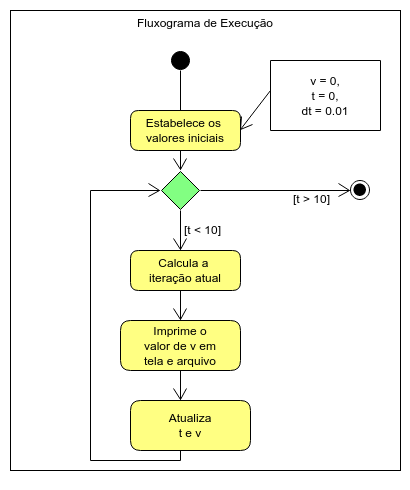
\includegraphics[width=10cm]{figuras/fluxograma.png}\\
  \caption{Fluxo de execução da solução}\label{fig:fluxo}
\end{figure}

A solução elaborada neste relatório funciona da seguinte maneira. Baseando-se nos valores iniciais fornecidos pela questão, o programa calcula os valores para a iteração atual, de acordo com o método de Runge-Kutta. Após isto é exibido o valor atual de $v$, então os valores são incrementados. Após isso, caso o limite máximo não tenha sido atingido, o programa executa o loop novamente.

\newpage
\section{Código Fonte}\label{sec:codigofonte}

\lstinputlisting[language=C]{../solution/m6.c}

\newpage
\section{Resultados e discussões}

Nesta seção discutiremos os resultados obtidos após a execução do programa apresentado na seção anterior. Abaixo é apresentada a plotagem do gráfico da equação~\eqref{eq:edo} para o intervalo $[0, 10]$, como havia sido estabelecido no início do relatório. Para gerar estes pontos, basta executar o programa. Um arquivo será gerado com todos os pontos e os respectivos valores. Então, através da ferramenta Gnuplot, foi feita a plotagem do gráfico, com os seguintes comandos:

\lstinputlisting[language=C]{figuras/graph.gnu}

\begin{figure}[!h]
  \centering
  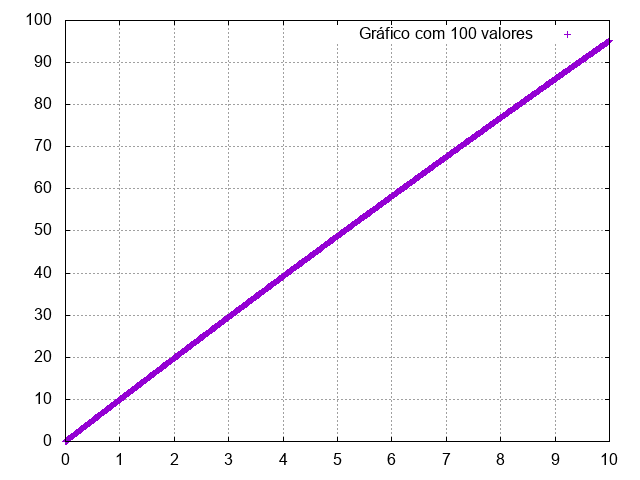
\includegraphics[width=12cm]{figuras/graph.png}\\
  \caption{Plotagem de 100 valores no intervalo $[0,10]$ }\label{fig:graph}
\end{figure}
\newpage

Abaixo, segue alguns dos resultados obtidos após a execução do programa. A solução proposta gera 1000 valores, devido a esta quantidade de resultados apenas alguns foram exibidos para comprovar o funcionamento da solução.
\begin{figure}[!h]
  \centering
  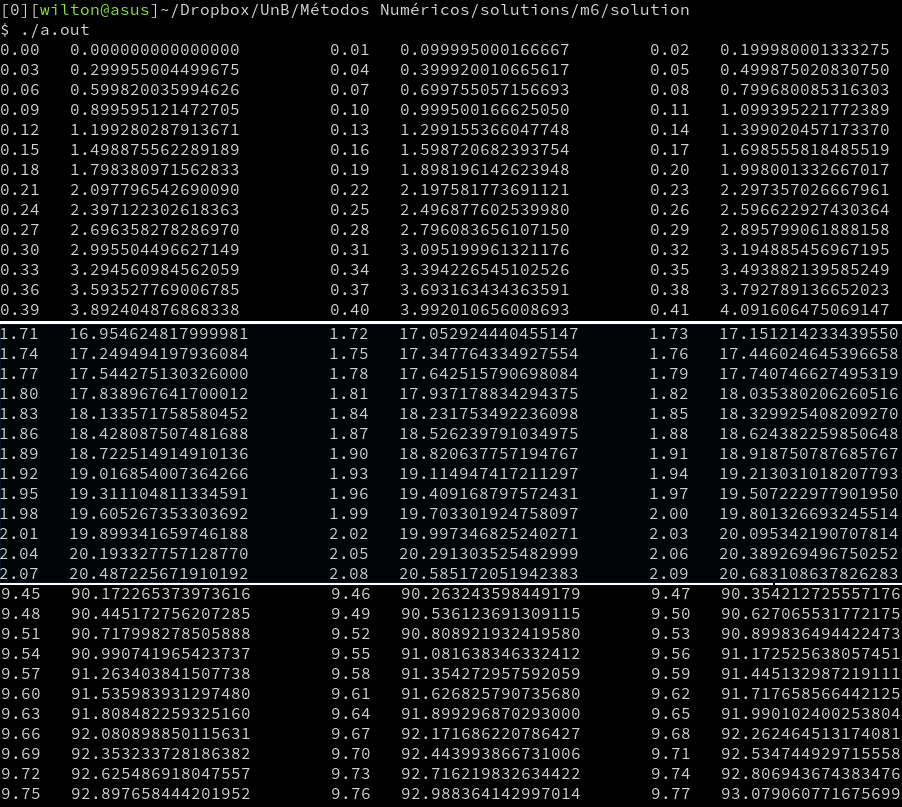
\includegraphics[width=15cm]{figuras/result.png}\\
  \caption{Alguns resultados da execução do programa}\label{fig:result}
\end{figure}

Sendo assim, o objetivo proposto no início do relatório foi satisfatoriamente alcançado.

\newpage
\section{Ferramentas}
Todas as ferramentas utilizadas neste relatório são ferramentas open source (software livre).
Permitindo assim que qualquer um possa reproduzir e contestar as afirmações presentes neste documento.

\begin{enumerate}
  \item Arch Linux (\url{https://www.archlinux.org})
    \begin{itemize}
      \item Sistema operacional utilizado.
    \end{itemize}
  \item GCC (\url{https://gcc.gnu.org})
    \begin{itemize}
      \item Compilador de C utilizado para compilar a solução.
    \end{itemize}
  \item Python (\url{https://www.python.org})
    \begin{itemize}
      \item Linguagem de programação utilizada para conferir os valores da solução.
    \end{itemize}
  \item vim (\url{http://www.vim.org})
    \begin{itemize}
      \item Editor de texto.
    \end{itemize}
  \item \LaTeX~(\url{https://www.latex-project.org})
    \begin{itemize}
      \item Sistema tipográfico de alta qualidade (utilizado para elaborar o relatório).
    \end{itemize}
  \item Gnuplot (\url{http://www.gnuplot.info})
    \begin{itemize}
      \item Utilitário de representação gráfica (utilizado para plotagem do gráfico).
    \end{itemize}
  \item UMLet (\url{http://www.umlet.com})
    \begin{itemize}
      \item Ferramenta de UML (utilizado para criar o fluxo de execução).
    \end{itemize}
  \item Shutter (\url{http://shutter-project.org})
    \begin{itemize}
      \item Programa de captura de tela (utilizado para capturar os resultados).
    \end{itemize}
\end{enumerate}

%%%%%%%%%%%%%%%%%%%%%%%%%%%%%%%%%%%%%%%%%%%%%%%%%%%%%%%%%%%%%%%%%%%%%%%%%%%%%%%%%%%%%%%%%

\end{document}
